\chapter{Interface Phonon Properties}

% \ifpdf
%     \graphicspath{{Chapter2/Figs/Raster/}{Chapter2/Figs/PDF/}{Chapter2/Figs/}}
% \else
%     \graphicspath{{Chapter2/Figs/Vector/}{Chapter2/Figs/}}
% \fi

\graphicspath{{Chapter3/}}
\setlength{\epigraphwidth}{0.6\textwidth}
\epigraph{“There are no real one-particle systems in nature, not even few-particle
systems. The existence of virtual pairs and of pair fluctuations shows that
the days of fixed particle numbers are over.”}
{\textit{Viki Weisskopf(American theoretical physicist)}}



\section[Introduction: Why we focus on interface]{Why we focus on interface}
\subsection{Research update: Heat conduction in nanostructured materials}  % also can get a short title like the \section
After we study the quasi-ballistic phonon transport in nano-films with MC method and get an overview of the temperature profiles in different 
knudsen Numbers, we have clearly observed the size effect caused by internal phonon scattering. And what should be pointed out is that in this former work we did not consider the effect of phonon boundary scattering in interfaces, but when it comes to actual device, multi-structured silicon devices have complex interfaces and experiments have demonstrated that in this regime, the surface or interface scattering becomes predominant compared to the internal scattering\cite{ChenRenkun,Hochbaum1}.\\
\indent Just as we have mentioned before, with the formidable and accelerated integration of transistor devices started in the sixties - about 9 billions CPUs are in function today - and the mid-heighties apparition of nanosciences, which finally benefited mostly to the materials
community, the question of the thermal management of small systems and of the micro-to-nanoscale thermal design of
materials led to the necessity of revisiting heat transfer principles\cite{Volz1}.
\\
\indent So we will turn to managment of multi-structured systems and focus on the phonon properties in interfaces. Althogh we employ the similarity of phonons and photons in our design of MC simulation algorithm, when it comes to the interface, phonons are more difficult to apprehend as they are non-local quasi-particles like photons\cite{zimanphonons}. Phonons
are strongly interacting together through inelastic or anharmonic three- or four-body interactions and there typical wavelength at room temperature remains lower than 10nm\cite{ChenRenkun} (whereas photon Wien’s wavelength is of ten microns). And in our focused regime, thermal wavelengths comparable to the system size lead to confinement, which in turn yields to a reduced phonon transport due to group velocity decrease but also to relaxation time modification\cite{kazan}.
\subsection{Status and Challenges:Multiscale phonon transport calculations}
In contrast to photonics, plasmonics or acoustics where a single mode can be excited and analyzed, the main difficulty in phonon heat conduction consists in the treatment of a broad band Planck’s spectrum reaching tens of TeraHertz where modes are thermally excited in all directions in the form of decorrelated wave packets strongly interacting together through complex selection rules. This challenging situation makes of heat conduction a very rich science involving solid-state, statistical, quantum and transport physics\cite{Volz1}.\\
\indent While the impact of surface and interface scattering has been shown\cite{VolzSeba}, the detailed descriptions of the phonon wave mechanisms occurring at the boundary remain to be established. Confinement effect, which was predicted\cite{Baltes,Montroll} before, has received strong proofs in nanowires, nanofilms\cite{kazan} and especially in superlattices\cite{Luckyanova,Ravichandran}.\\
\indent One important breakthrough to model  realistic phonon properties such as relaxation times is based on the DFT(density functional theory) approaches\cite{Ward}.
Compared with the MD method\cite{Ladd,Volz2} which has been widely used before and depends on the validity of the interatomic pseudopotential,the DFT method represents quantum populations and is discarding the contribution of free electrons.
However, the estimations remain limited to periodic or few atoms systems and also adopt many approximations such as single mean relaxation time and local near-to-equilibrium approximations. And this is why we choose to use classical potential to perform our calculations in later work, because doing calculations based on DFT is rather time-consuming, especially for lager systems. And also we will give a short introduction on Quantitative calculation from first principles based on density functional theory to compare with our AGF method based on the classical potential in Appendix2.


%\section*{Enumeration}
\section[Methodology: The Atomistic Green,s Function Method]{AGF: The Methodology}
\subsection{Introduction}
A growing interest exists in mesoscopic phonon transport, in which device dimensions becomes comparable to the typical wavelength of a phonon, and the wave nature of phonons becomes prominent. And as we have discussed above, phonon transport is often restricted by the heterogeneous boundaries and interfaces embedded in devices.In this quasi-ballistic transport regime, the atomistic Green’s function (AGF) method is efficient at handling interface and boundary scattering\cite{ATF}. The atomistic Green’s function approach combines atomic-scale fidelity with asymptotic treatment of large-scale (bulk) features, such that the method is particularly well suited to address an emerging class of multiscale transport problems\cite{ReviewATF}.\\
\indent Compared to other methods such as molecular dynamics (MD)\cite{MD1,MD2} and the phonon Boltzmann transport equation (BTE)\cite{BTE1,BTE2}, the atomistic Green’s function method is strictly valid at low temperatures. It accounts for boundary and interface scattering efficiently and offers great flexibility in handling complicated geometries\cite{ATF}.\\
\indent To set up a correct configuration we should notice that in a typical device-contact setup, contacts (or thermal reservoirs) play significant roles. Phonon distributions in contacts can significantly change the phonon transport characteristics of the device\cite{Angelesc}. That can be strictly met in AGF method because the AGF method uses self-energy matrices to represent the effect of bulk contacts on the device, thus simplifying the complexities of multiscale transport.\\
\indent One last thing before we turn to the details of the AGF method is that we need to know the two primary theories that have been employed to explain the mechanism of the thermal boundary resistance.One is the acoustic mismatch model (AMM)\cite{AMM}, and the other is the diffuse mismatch model (DMM)\cite{DMM}. Both models neglect atomic details of actual interfaces, and thus offer limited accuracy in nanoscale interface resistance predictions\cite{Stevens}. The AGF method can predict thermal boundary resistance between heterogeneous materials with full consideration of the interfacial atomic structures. And we will return to this topic in 3.4 and 3.5 when we consider and study detailedly on the ITC(interfacial thermal conductance)\\
\indent In the following part, a detailed mathematical
derivation of the phonon transmission function is provided in terms of Green’s functions and, using the transmission function, the heat flux integral is written in Landauer form. Within this theoretical framework, the required inputs to calculate heat flux are equilibrium atomic locations and an appropriate interatomic potential.

\subsection{AGF:Mathematical Formation}
\subsubsection*{General Description}
 First let us take a look at the common atomic structure of interest, which can be generalized as a device between two contacts, as shown in Fig\ref{fig:contact}.As is shown in the fig, Contact1(separated into two atom groups LCB and LC) and Contact2(separated into two atom groups RCB and RC) are two semi-infinite thermal reservoirs at constant temperature $T_1$ and $T_2$, respectively.And the Device includes three atom groups LD,D and RD, what is important is its geometry is arbitrary, which means it can be an atomic chain or a nanowire even a nanofim.\\
\indent The other thing about the setup is the connections.The types of connections between the device and contacts are arbitrary(point contact, limited contact or planar contact). And the difference between LCB and LC is atom group LC includes atoms that bond with Device atoms while LCB doesn't.That will bring out the difference of the dynamical properties of these two groups, LC and LCB in general heterogeneous system. And the bonds connection is the same at the right end. 


\begin{figure}[htbp!] 
\centering    
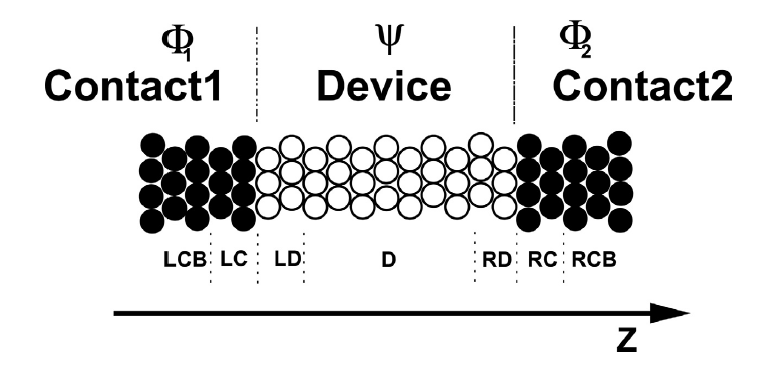
\includegraphics[width=0.6\textwidth]{contact}
\caption[contact]{Schematic diagram for a general contact-device-contact setup\cite{ATF}}
\label{fig:contact}
\end{figure}

\subsubsection*{Harmonic Matrix}
The AGF method\footnote{We mainly list the important formulas and omit the mathematical derivation} is founded on a harmonic matrix of the system of interest. Because prior work has shown that anharmonic scattering can generally be neglected at room temperature when the characteristic length of the device is less than 20 nm and we are focusing on atomistic structure of interface which usually consists of tens to hundreds of atoms, a harmonic matrix can be used to represent interactions among different degrees of freedom.The definition of the harmonic matrix in math is as follows\footnote{We use no Einstein summation rule in this article}
\begin{equation}
\textbf{H}={H_{pq}}=\frac{1}{\sqrt{M_p M_q}}\left\{\begin{array}{ll}
-\frac{\partial^2 U}{\partial U_p \partial U_q}&  \text{if p $\neq$ q},\\
-\sum_{m \neq q} -\frac{\partial^2 U}{\partial U_p \partial U_m} & \text{if p = q}.
\end{array}\right. \label{con:harmonic}
\end{equation}\\
In which $u_p$ and $u_q$ refer to any two atomic virational degrees of freedom (displacements,
momentums),respectively.U represents the total interatomic potential. What should be noticed, $M_p$ and $M_q$ are atomic masses associated with degrees of freedom $u_p$ and $u_q$. \\
Therefore, according to Solid Physics\cite{Ashcroft},the dynamic equation for the system can take this form
\begin{equation}
(\omega^2 \textbf{I}-\textbf{H})\tilde{u} = 0 \label{con:dynamic} 
\end{equation}\\
Where $\tilde{u}$ is a column vector consisting of vibrational degrees of freedom.And we note that though the assembled matrix $\textbf{H}$ can contain complex entries in complicated situations, its being Hermitian matrix guarantees that it has only real eigenvalues.

\subsubsection*{Green's Function Matrices}
Matrices $\tau_1$ and $\tau_2$ are used to represent interactions between two different atom groups. And the column vector $\psi$ and $\phi$, which can be seen in Fig\ref{fig:contact}, represent vibrational degrees of freedom in the device in contacts. We need to know that the number of degrees of freedom in the contact approaches infinity, so we use a sufficiently large number $n_c$ to approximate the number.$n_d$ and $n_c$ are degrees of freedom in the device and in interface regions(LC,LD,RC and RD).\\
We can derive the dynamic equations of the disconnected contacts based on Eq(\ref{con:dynamic})
\begin{equation}
[\omega^2 \textbf{I} - \textbf{$H_1$}] \phi_1^R=0
\end{equation}
\begin{equation}
[\omega^2 \textbf{I} - \textbf{$H_2$}] \phi_2^R=0
\end{equation}
where $\textbf{$H_1$}$ and $\textbf{$H_2$}$ are harmonic matrices of the two contacts.The superscript R means the disconnected state. We next use $\chi$ to denote the change to the original contact vector($\phi^R$), so after the contact and device establishes the connection, the actual contact vector becomes $\phi=\phi^R + \chi$.
Now the dynamic equation can be written together in matrix form:
\begin{equation}
\left[
\begin{matrix}
\omega^2 \textbf{I} - \textbf{$H_1$}&-\tau_1^{\dag}&0&\\
-\tau_1&\omega^2 \textbf{I} - \textbf{$H_d$}&-\tau_2&\\
0&-\tau_2^{\dag}&\omega^2 \textbf{I} - \textbf{$H_2$}&
\end{matrix}
\right]
\left(
\begin{matrix}
\phi_1^R + \chi_1\\
\psi\\
\phi_2^R + \chi_2
\end{matrix}
\right) = 0 \label{con:connect} 
\end{equation}\\
We can write the solution to Eq(\ref{con:connect}):
\begin{equation}
\chi_1=g_1\tau_1^{\dag}\psi
\end{equation}
\begin{equation}
\chi_2=g_2\tau_2^{\dag}\psi
\end{equation}
\begin{equation}
\psi=GS
\end{equation}
And the matrices$g_1$,$g_2$,G and S are defined next:
\begin{equation}
g_1=\lim_{\delta \to 0}[(\omega^2 + \delta i) \textbf{I} - \textbf{$H_1$}]^{-1} \quad (uncoupled\quad Green's\quad Function)
\label{con:g1} 
\end{equation}
\begin{equation}
g_2=\lim_{\delta \to 0}[(\omega^2 + \delta i) \textbf{I} - \textbf{$H_2$}]^{-1} \quad (uncoupled\quad Green's\quad Function)
\label{con:g2} 
\end{equation}
\begin{equation}
G=[\omega^2 \textbf{I} - \textbf{$H_d$}-\tau_1 g_1 \tau_1^{\dag}-\tau_2 g_2 \tau_2^{\dag}]
\end{equation}
\begin{equation}
S=\tau_1\phi_1^R+\tau_2\phi_2^R
\end{equation}
And we use $\sum_1$ and $\sum_2$ to denote $\tau_1 g_1 \tau_1^{\dag}$
and $\tau_2 g_2 \tau_2^{\dag}$,$S_1$ and $S_2$ to denote$\tau_1\phi_1^R$and$\tau_2\phi_2^R$.\\
Several matrices used later for convenience are defined as
\begin{equation}
A=i[G-G^{\dag}]=i[g_1-g_1^{\dag}]+i[g_2-g_2^{\dag}]=G\Gamma_1G^{\dag}+G\Gamma_2G^{\dag}
\end{equation}
\begin{equation}
\Gamma=\tau_1A_1\tau_1^{\dag}+\tau_2A_2\tau_2^{\dag}
\end{equation}
Where the first term and the second term of A can be denoted as $A_1$ and $A_2$, while the same with $\Gamma$,namely,$\Gamma_1$ and $\Gamma_2$.
In Eq(\ref{con:g1}) and Eq(\ref{con:g2}),i is the unitary imaginary number.And perturbation $\delta$ is very important and will be discussed next.
\subsubsection{Energy Flux Between any Two Degrees of Freedom}
The energy associated with any degree of freedom consists of kinetic and potential energies,
\begin{equation}
E_p=\frac{1}{4}\sum_q (u_p^*k_{pq}u_q+u_q^*k_{qp}u_p)+\frac{M_p}{2}\dot{u_p^*}\dot{u_p}\label{con:energy}
\end{equation}
where
\begin{equation}
k_{pq}=H_pq\sqrt{M_p M_q}
\end{equation}
Using Newton's second law, we can get the time derivative of this energy($E_p$) and simplify it to this form, which is a typical form of an energy conservation equation
\begin{equation}
\frac{d E_p}{d t}=\frac{\omega}{2 i}\sum_q[\phi_p^* H_{pq} \phi_q - \phi_q^* H_{qp} \phi_p]\equiv \sum_q J_{pq}
\end{equation}
And $J_{pd}$ is natural to be defined as the energy flux between any two degrees of freedom($u_q$and$u_p$)
\begin{equation}
J_{pq}=\frac{\omega}{2 i}[\phi_p^* H_{pq} \phi_q - \phi_q^* H_{qp} \phi_p]\label{con:flux}
\end{equation}
And intuitively, we find the Eq(\ref{con:flux}) takes a very similar form of the energy flux in quantum mechanics derived from the schrodinger equation, which can partly prove the validity of the result. 
\subsubsection*{Normalization}
Using Eq(\ref{con:energy}) and $u_p=\phi_p \exp^{-i\omega t} /\sqrt{M_p}$,the normalization condition for phonons can be expressed as
\begin{equation}
\hbar \omega = \sum_p E_p = \sum_p \omega^2 |\phi_p|^2
\end{equation}
\subsubsection*{The Expression for Total Energy}
Total energy flux is obviously the summation of fluxes between individual degrees of freedom according to Eq(\ref{con:flux}),so, 
we write the heat flux between Contact1 and Device\footnote{We use the fact that the trace of any matrix product is independent of the order of multiplication}
\begin{equation}
J_1=\frac{\omega Trace [\psi^{\dag}\tau_1\phi_1 - \phi_1^{\dag}\tau_1^{\dag}\psi]}{2 i}=
\frac{\omega Trace [\psi^{\dag}\tau_1\phi_1^R - \phi_1^{R \dag}\tau_1^{\dag}\psi]}{2 i}+
\frac{\omega Trace [\chi_1^{\dag}\tau_1^{\dag}\psi - \psi^{\dag}\tau_1\chi_1]}{2 i}
\end{equation}
where the first and second term means the Inflow and Outflow.
We can write down $J_1$ similarly and after several derivations we can finally arrive at the Landauer form\citep{Buldum}:
\begin{equation}
J=\int \frac{\hbar \omega}{2 \pi}\Xi(\omega)[N_1(\omega)-N_2(\omega)]d\omega
\end{equation}
At the same time, we get the transmission function
\begin{equation}
\Xi(\omega)= Trace[\Gamma_1 G \Gamma_2 G^{\dag}]= Trace[\Gamma_2 G \Gamma_1 G^{\dag}]
\end{equation}
And the thermal conductance($\sigma$) is the ratio of heat flux J to the temperature difference
\begin{equation}
\sigma=\frac{J}{\Delta T}
\end{equation}

\subsubsection*{Several Points for Numerical Implementation}
First, we will talk about the algorithm and how to conduct the simulation based on the math:
\begin{enumerate}
\item The first step involves constructing harmonic matrix based on Eq\ref{con:harmonic}
\item The evaluation process can be conducted either by numerical(when potential is complicated) or analytical(when potential is simple), only if atomic locations and interatomic potential parameters are know.
\item Next we just need to calculate the uncoupled Green's functions $g_1$ and $g_2$.
\end{enumerate}
Another issue is the selection of $\delta$, which is a small number corresponding to phonon energy dissipation in contacts,whose role is elaborated in S. Datta's book\cite{Datta}.And according to former reference, it is recommended that $\delta$ can take the following general form\cite{ATF}:
\begin{equation}
\delta=f(\omega) \omega^2
\end{equation}
where $f(\omega)$ is a monotonically decreasing function.
The choice of $\delta$ affects the energy resolution in the uncoupled Green's function and subsequent calculations\cite{ReviewATF}. A small $\delta$ value gives better energy resolution but also needs longer computational time.

\section{Phonon properties of interfaces across III-V semi-conductors}

\subsection{The Area Effect on transmittance and the Convergence}
As for the phonon transmittance in interface, it is not hard to derive that it couldn't depend on the size of the interface and it should only depend on the types of structures of interface.But in actual calculations, as a result of several factors, we can observe that the results may change as the the size of interface changes. So that the problem we need to handle before we begin our calculations, namely, we need to figure out the smallest size of the interface to get the stable result('smallest' means we can save the cost of simulation).\\
\indent So we conduct a series of simulations of two types of system, one is the Si-Ge interface the other the GaP-GaAs interface. We calculate the phonon transmittance of several sizes of interfaces, ranging from 1x1 to 10x10(Which is perpendicular to the Z direction which is the heat flux direction).\\
\indent Where Fig(\ref{fig:Gaa}) and Fig(\ref{fig:Gab}) show the transmittance of different sizes of GaP/GaAs while Fig(\ref{fig:Gaa}) and Fig(\ref{fig:Gab}) show that of Si/Ge. It is clearly shown that only if the area is large enough will the transmittance be convergent, and we later will choose the 8x8 size for our calculation.
\begin{figure}
\begin{minipage}[t]{0.5\linewidth}
\centering
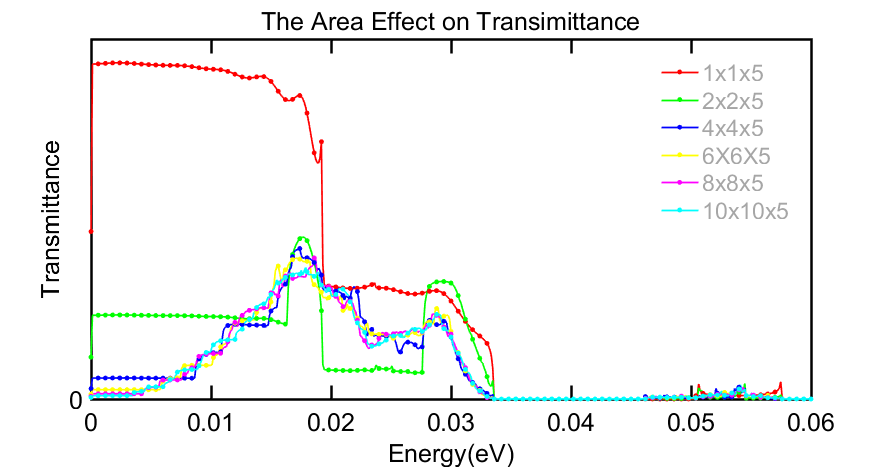
\includegraphics[width=\textwidth]{GaPGaAs_Big.png}
\caption{GaP/GaAs(a)(Colored online)}
\label{fig:Gaa}
\end{minipage}%
\begin{minipage}[t]{0.5\linewidth}
\centering
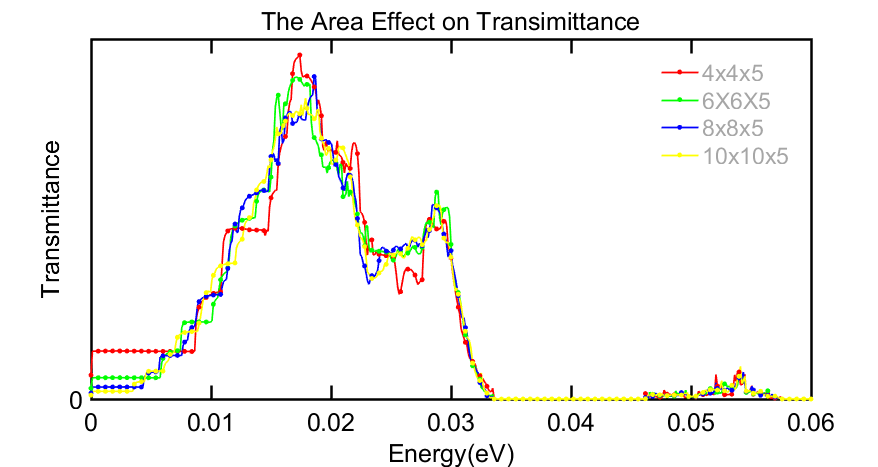
\includegraphics[width=\textwidth]{GaPGaAs_sub.png}
\caption{GaP/GaAs(b)(Colored online)}
\label{fig:Gab}
\end{minipage}
\end{figure}
\par
\hspace{-0.2in}
\begin{figure}
\begin{minipage}[t]{0.5\linewidth}
\centering
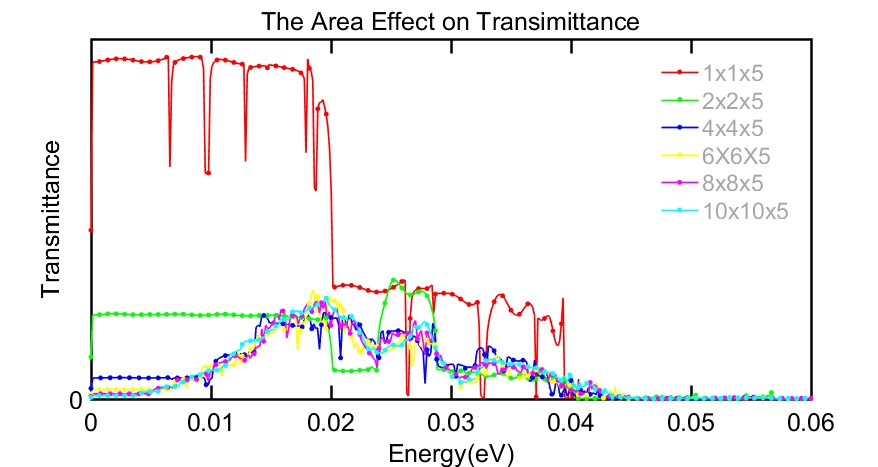
\includegraphics[width=\textwidth]{SiGe_Big.png}
\caption{Si/Ge(a)(Colored online)}
\label{fig:SiGea}
\end{minipage}%
\begin{minipage}[t]{0.5\linewidth}
\centering
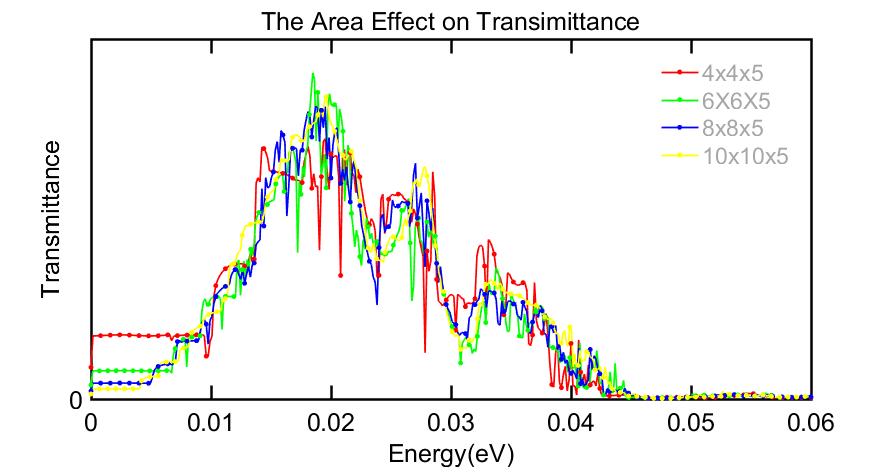
\includegraphics[width=\textwidth]{SiGe_sub.png}
\caption{Si/Ge(b)(Colored online)}
\label{fig:SiGeb}
\end{minipage}
\end{figure}
\subsection{The Optimization of Interface and Device}
After we construct a interface and then get a device for AGF calculation, the first thing we should do is to relax the configuration to lower its total energy. We give a detailed description of the optimization methods we adopt in  \textbf{Appendix C}, and here we will give the example of the optimization of GaN/GaP interface.\\
\indent The crystal structure of GaN is Wurtzite, while the GaP is Zincblende type. Considering that they have the different types of crystal structures, it is a perfect example to explain the optimization process.\\
\indent As shown in the Fig(\ref{fig:centralop}) and Fig(\ref{fig:1DMINop}), the total energy of the whole system becomes lowers as the iteration steps grow and the stress also becomes stable.
\begin{figure}
\begin{minipage}[t]{0.5\linewidth}
\centering
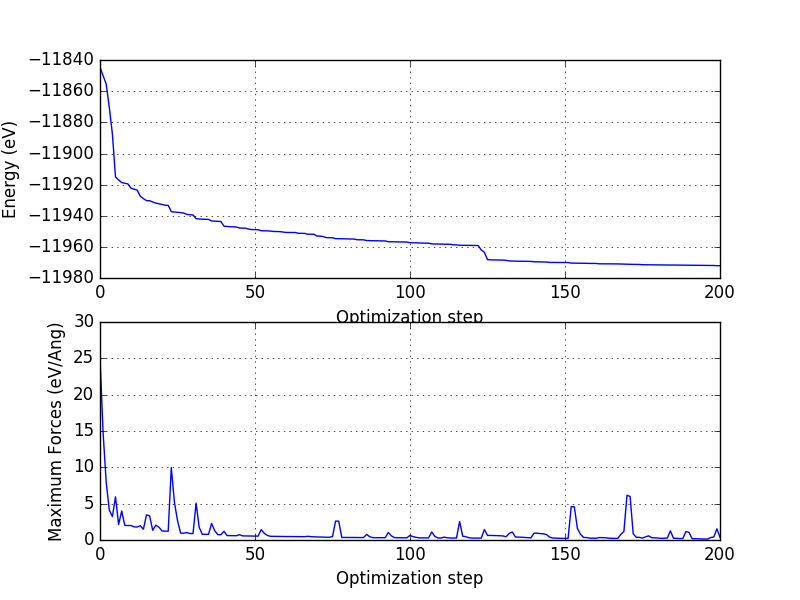
\includegraphics[width=\textwidth]{central.png}
\caption{The central region optimization with rigid ends}
\label{fig:centralop}
\end{minipage}%
\begin{minipage}[t]{0.5\linewidth}
\centering
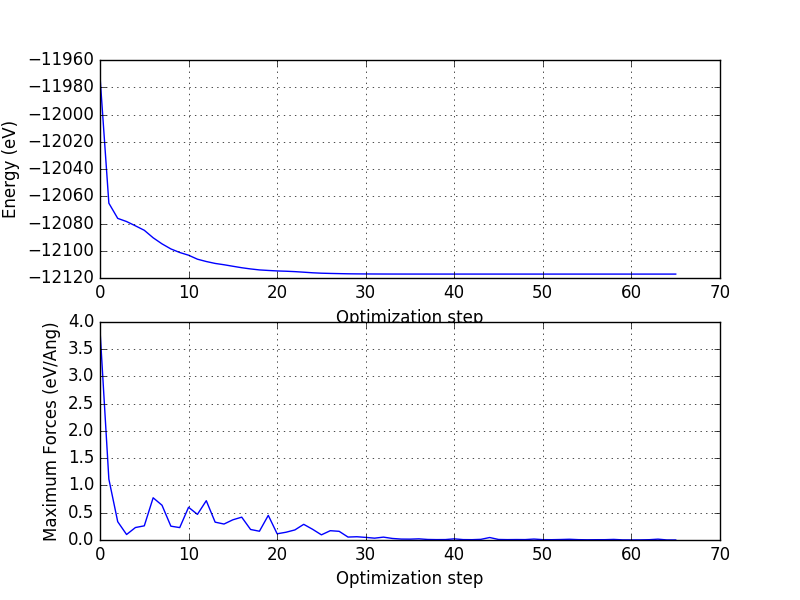
\includegraphics[width=\textwidth]{1DMIN.png}
\caption{1DMIN of the whole device}
\label{fig:1DMINop}
\end{minipage}
\end{figure}

\subsubsection*{The layers of interface}
We use rigid constraints at both ends so the layers of atoms in the interface region can have an effect on the result. We test the different layers of atoms with Si/SiC and it can be clearly shown in Fig(\ref{fig:length1}) and Fig(\ref{fig:length2}), the result becomes consistent when layers are thick enough, so we use four layers in our calculations.
\begin{figure}
\begin{minipage}[t]{0.5\linewidth}
\centering
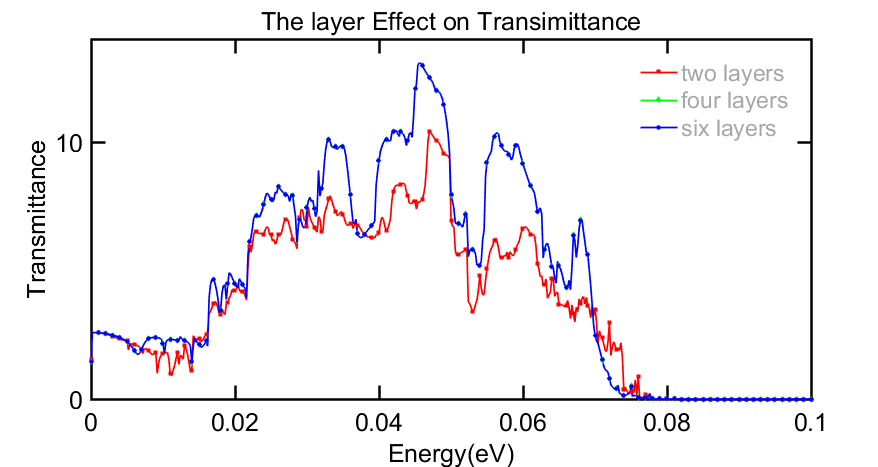
\includegraphics[width=\textwidth]{length1.png}
\caption{Si/Sic (Colored online)}
\label{fig:length1}
\end{minipage}%
\begin{minipage}[t]{0.5\linewidth}
\centering
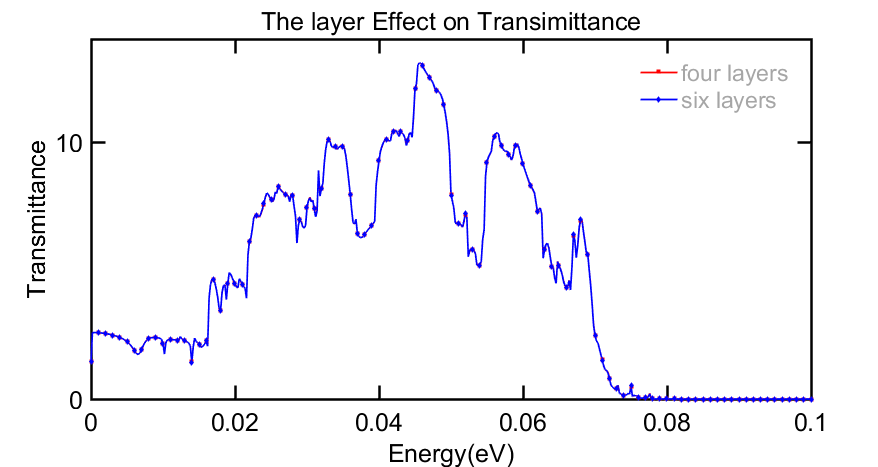
\includegraphics[width=\textwidth]{length2.png}
\caption{Si/SiC interface(four and six)(Colored online)}
\label{fig:length2}
\end{minipage}
\end{figure}
\subsection{Calculation Details}
As we have discussed in \textbf{3.2}, for AFG calculation, the input is the configuration information(the type and the initial position of atoms) and the interaction. The former can be given after we get the device configuration(after optimization), and the former we need define the interaction potential or give from first principle or others. \\
\indent We choose the Tersoff potential given by blabla in our AGF work. The details and a brief introduction to Tersoff potential is in\textbf{Appendix C}. Here we will give the reason why we choose the empirical potential instead of the first principle method:
\begin{itemize}
\item The Tersoff type potential\cite{TeroffIIIV} we use is specifically set for the III-V seimi-conductors and has been proved effective in several works\cite{tersoffwork1,tersoffwork2,teroffwork3,tersoffwork4}.
\item Although several improvements have been made in first principle calculations, the simulation of a system like ours can still be very time-consuming. Just use $Si/SiO^2$ for example, if we use empirical potential to optimize the device it usually cost less than a minute while for first principle calculation it can cost more than a hour if both run on a PC. And that is just the optimization process so even though we use
parallel computing, the first principle cannot been acceptable.
\end{itemize}
\subsubsection*{The bandstructure and the Phonon Density of States(DOS)}
Before we begin to analyze our AGF results, it is essential  to calculate the phonon bandstructure and Density of States, which can inspire our late insight on AGF results.

\begin{figure}

\centering
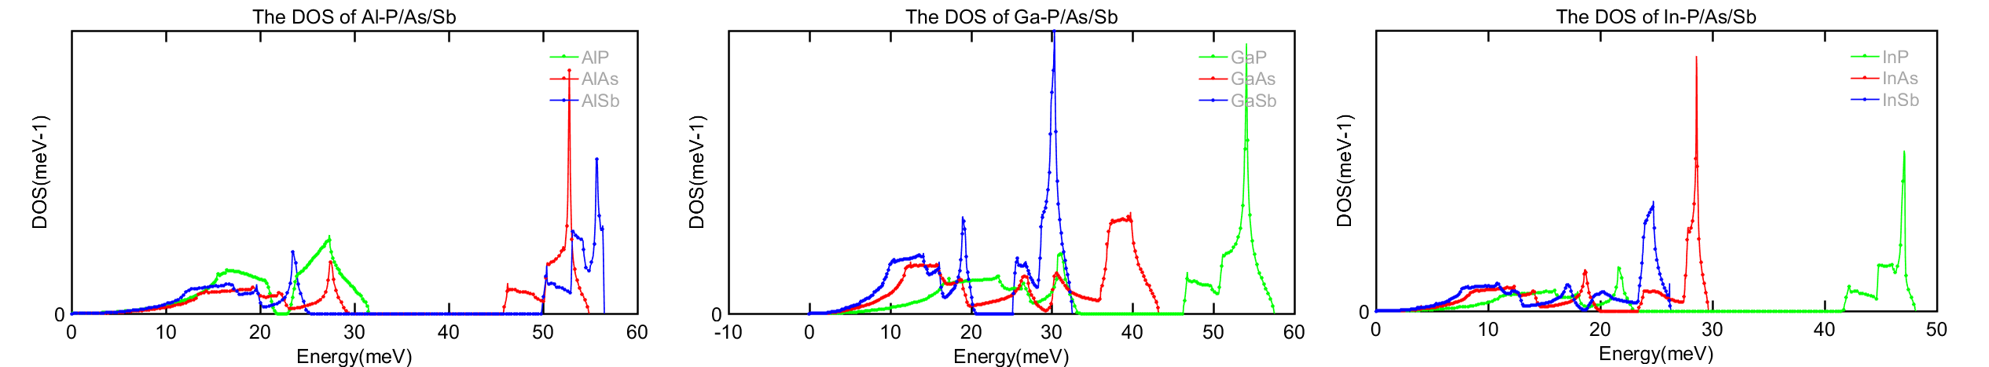
\includegraphics[width=\textwidth]{dos.png}
\caption{DOS(Colored online)}
\label{fig:dosall}
\end{figure}

\subsection{Results}
In real materials, the lattice constants
of the materials across interfaces are often different, and
lattice mismatch could result in atomic reconstruction in
the interfacial region. Such interfacial reconstruction can
change the phonon transmission at the interface and thus
the interfacial thermal conductance. In most of the past works, this effect is ignored but in our work we exploit a relaxation way to cope with this effect.\\
\indent In this section, phonon transmission across a single interface between two semi-infinite III-V semi-conductors as shown in Fig(\ref{fig:TAlP},\ref{fig:TAlAs},\ref{fig:TAlSb}) is studied. As we studied 9 types of III-V semi-conductors in all, so the combinations can be 36, we just show part of the results(Transmittance of AlX(X=P,As,Sb), for example.).

\begin{figure}
\centering
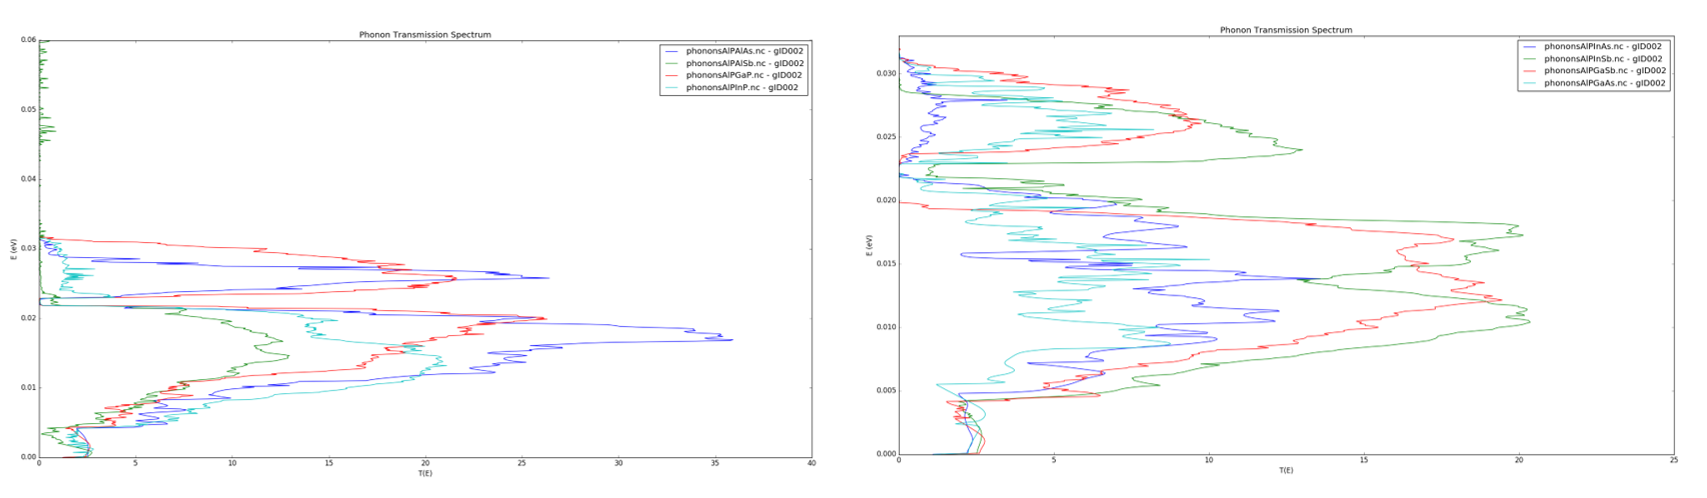
\includegraphics[width=\textwidth]{AlP.png}
\caption{Phonon transmission across a single interface of bulk AlP and other materials(Colored online)}
\label{fig:TAlP}
\end{figure}

\begin{figure}

\centering
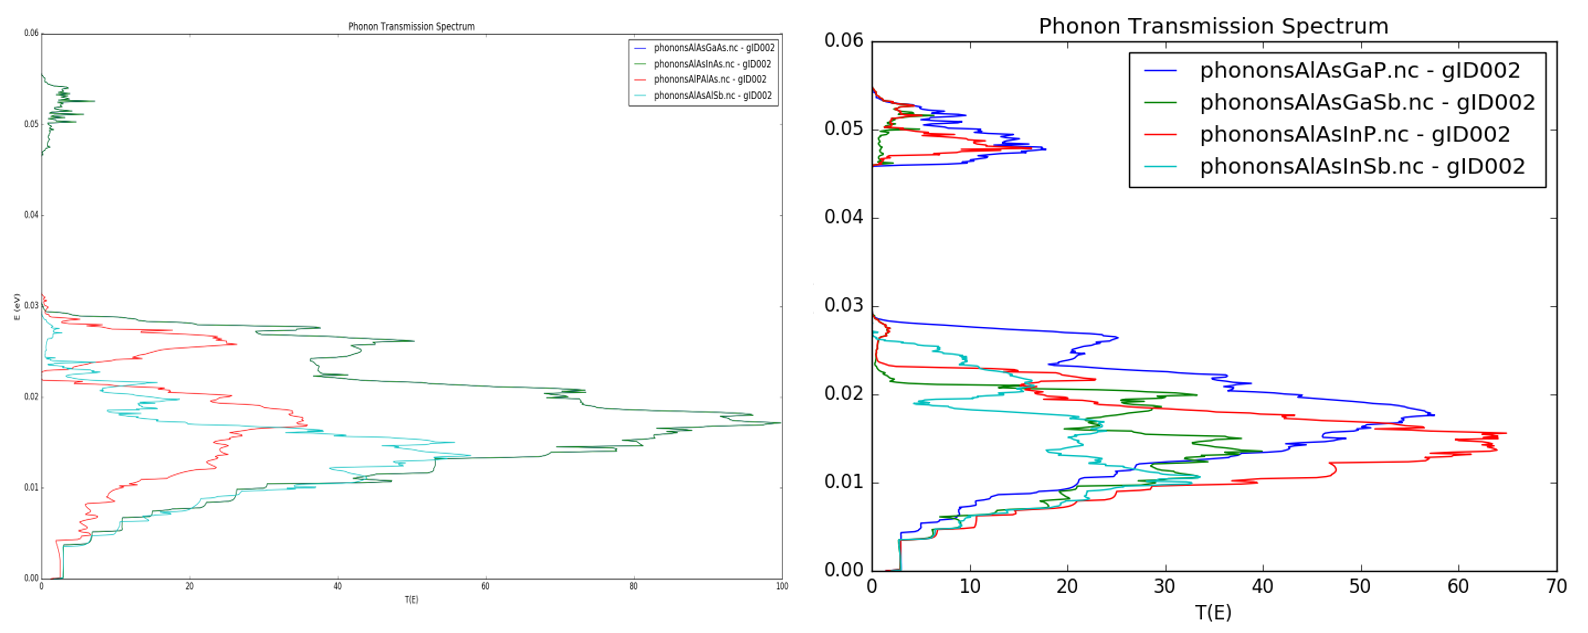
\includegraphics[width=\textwidth]{AlAs.png}
\caption{Phonon transmission across a single interface of bulk AlAs and other materials(Colored online)}
\label{fig:TAlAs}
\end{figure}%

\begin{figure}

\centering
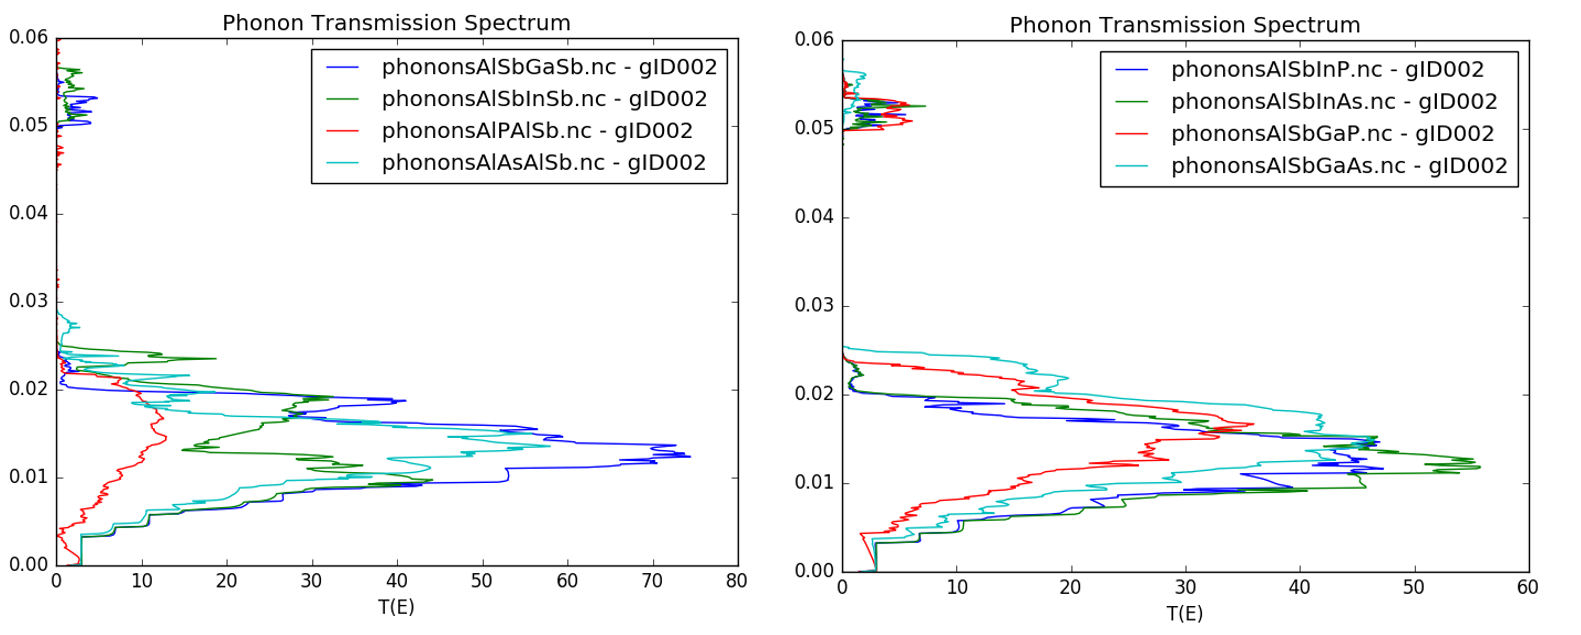
\includegraphics[width=\textwidth]{AlSb.png}
\caption{Phonon transmission across a single interface of bulk AlSb and other materials(Colored online)}
\label{fig:TAlSb}
\end{figure}%

\subsection{Discussion}
We studied the phonon transmission across GaP/GaAs, GaP/GaSb and GaAs/GaSb for example, and the results are shown in Fig(\ref{fig:TGa}). In the low frequency region, there are more similarity with GaP and GaAs in dos, so the transmittance is large while in the high frequency region, the bigger difference in dos caused a low transmittance. And also when the atoms become bigger(heavier), the peak of transmission goes to the lower frequency region, which may be explained by the dominating phonons(having the main percent of energy) change.\\
\indent Here we just give a short and brief discussion of this issue, and we will return to this topic in the later Chapter and also this will be the core focus of our later work.

\begin{figure}

\centering
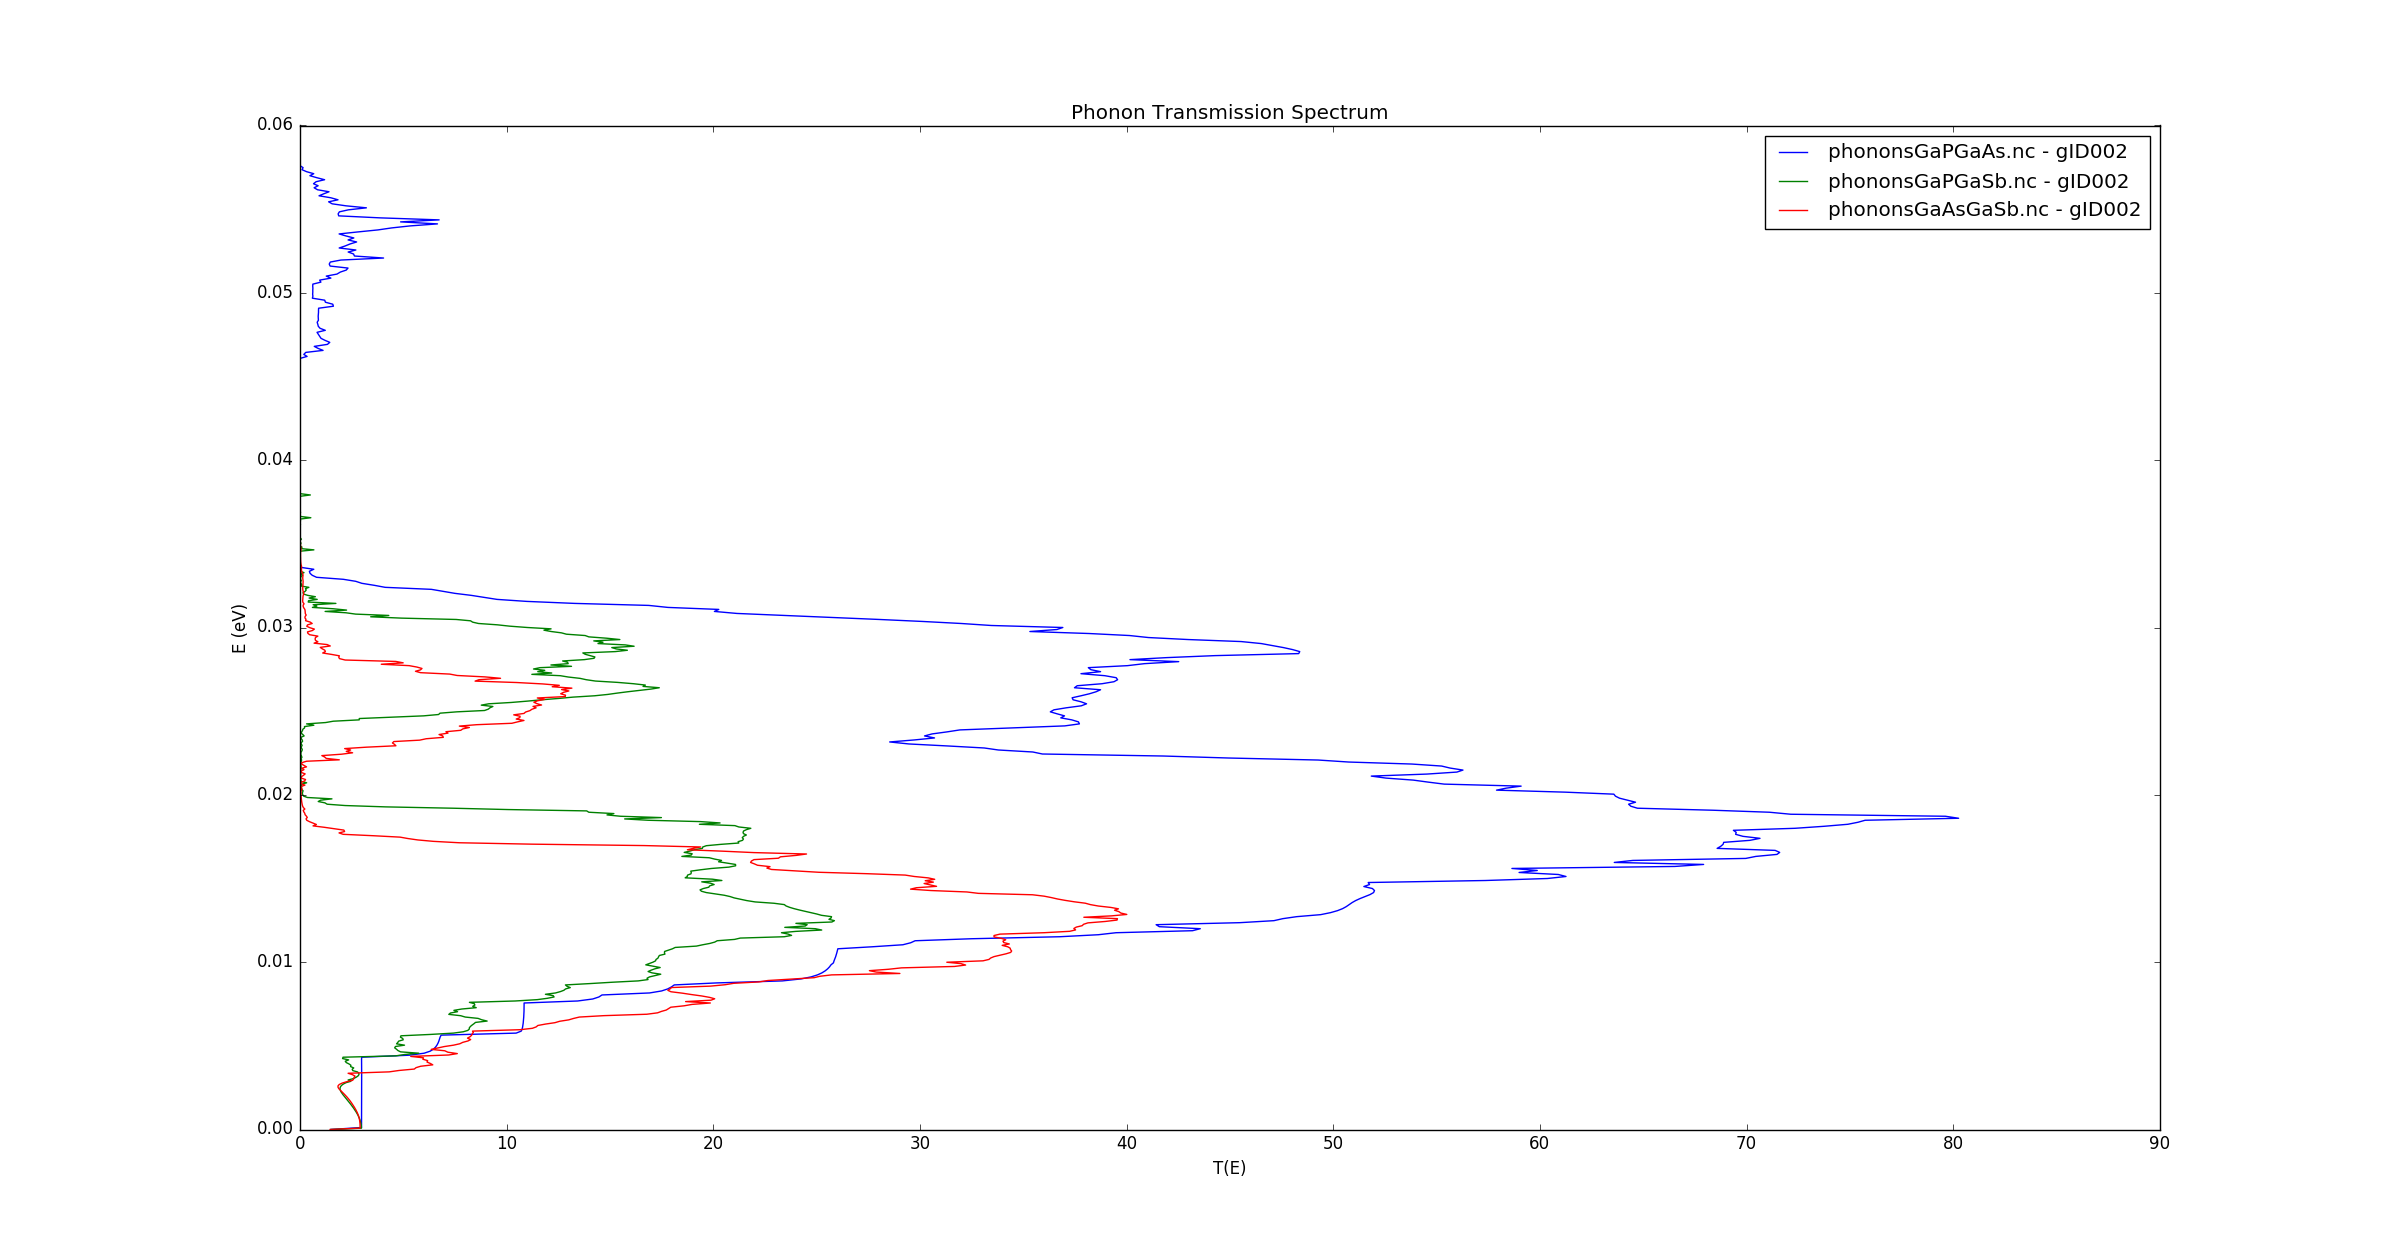
\includegraphics[width=\textwidth]{TGa.png}
\caption{Phonon transmission across a single interface of bulk GaP,GaAs and GaSb(Colored online)}
\label{fig:TGa}
\end{figure}%

\nomenclature{g}{uncoupled green's function matrix}%
\nomenclature{G}{green's function matrix}%
\nomenclature{$\hbar$}{reduced Planck constant(=$h/2\pi$)}%
\nomenclature{\textbf{H}}{harmonic matrix}%
\nomenclature{i}{unitary imaginary number}%
\nomenclature{\textbf{I}}{identity matrix}%
\nomenclature{J}{energy flux}%
\nomenclature{$k_B$}{Boltzmann constant(=1.38 $\times$ $10^{-23}$ kg/$s^2$k)}%
\nomenclature{M}{atomic mass}%
\nomenclature{S}{source matrix}%
\nomenclature{t}{time}%
\nomenclature{i}{unitary imaginary number}%
\nomenclature{A}{matrix for convenience}%
\nomenclature{$\Gamma$}{matrix for convenience}%
\nomenclature{$\tilde{u}$}{column vector consisting of vibrational degrees of freedom}%
\nomenclature{U}{interatomic potential}%
\nomenclature{$\delta$}{a small number corresponding to phonon energy dissipation in contacts}%
\nomenclature{$\sigma$}{thermal conductance (W/K)}%
\nomenclature{$\omega$}{angular frequency(rad/s)}%
\nomenclature{$\sum$}{self-energy matrix}%
\nomenclature{$\tau$}{matrix representing interactions}%
\nomenclature{$\phi$}{column vector representing vibrational degrees of freedom in either contact}%
\nomenclature{$\chi$}{column vector representing the change to the original vector $\phi^R$ after contacts and the device are connected}%
\nomenclature{$\psi$}{column vector representing vibrational degrees of freedom in the connected device}%







 
\nomenclature{LCB}{left contact bulk region}%
\nomenclature{LC}{left contact region}%
\nomenclature{LD}{left device region}%
\nomenclature{RCB}{right contact bulk region}%
\nomenclature{RC}{right contact region}%
\nomenclature{RD}{right device region}%
\nomenclature{d}{device region including LD,RD and D}%
\nomenclature{m}{degree of freedom running index}% 
\nomenclature{p}{matrix row index, or the index of a degree of freedom}%
\nomenclature{q}{matrix row index, or the index of a degree of freedom}%
\nomenclature{R}{disconnected state}%
\nomenclature{*}{complex conjugate of a matrix}%
\nomenclature{$\dag$}{conjugate transpose of a matrix}%
\printnomenclature   %%% 出现的地方
 



\clearpage
